\documentclass{article}
\usepackage{tikz}

\begin{document}

\begin{figure}[h]
    \centering
    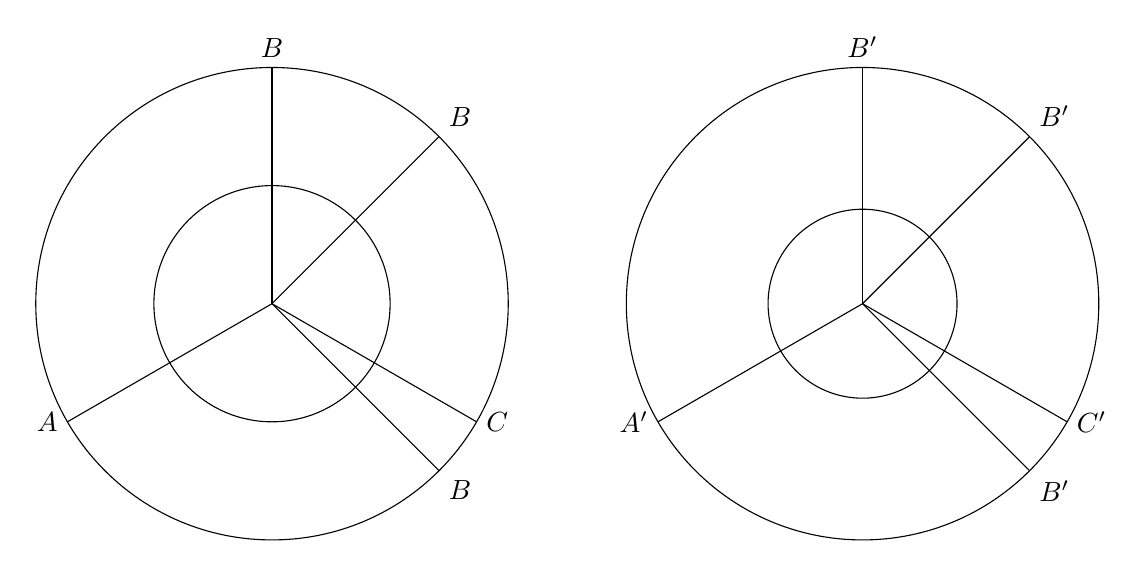
\begin{tikzpicture}[scale=1.5]

        % Diagram (a)
        \draw[fill=white] (0,0) circle (2cm);
        \draw[fill=white] (0,0) circle (1cm);

        \draw (0,0) -- (90:2cm) node[above] {$B$};
        \draw (0,0) -- (210:2cm) node[left] {$A$};
        \draw (0,0) -- (330:2cm) node[right] {$C$};
        \draw (0,0) -- (45:2cm) node[above right] {$B$};
        \draw (0,0) -- (-45:2cm) node[below right] {$B$};

        % Diagram (b)
        \begin{scope}[xshift=5cm]
            \foreach \r in {0.8, 1.2, 1.6, 2.0} {
                \draw[fill=white] (0,0) circle (\r cm);
            }
            \draw[fill=white] (0,0) circle (0.8cm);

            \draw (0,0) -- (90:2.0cm) node[above] {$B'$};
            \draw (0,0) -- (210:2.0cm) node[left] {$A'$};
            \draw (0,0) -- (330:2.0cm) node[right] {$C'$};
            \draw (0,0) -- (45:2.0cm) node[above right] {$B'$};
            \draw (0,0) -- (-45:2.0cm) node[below right] {$B'$};
        \end{scope}

    \end{tikzpicture}
    \caption{(a) A simple diagram with sectors. (b) A more complex diagram with concentric circles.}
    \label{fig:sample_550}
\end{figure}

\end{document}